\begin{frame}[t]{ALTERNATIVMETHODE}
  \begin{columns}
    \begin{column}{0.5\textwidth}
      Cuts auf Farbkanälen

      \centering
      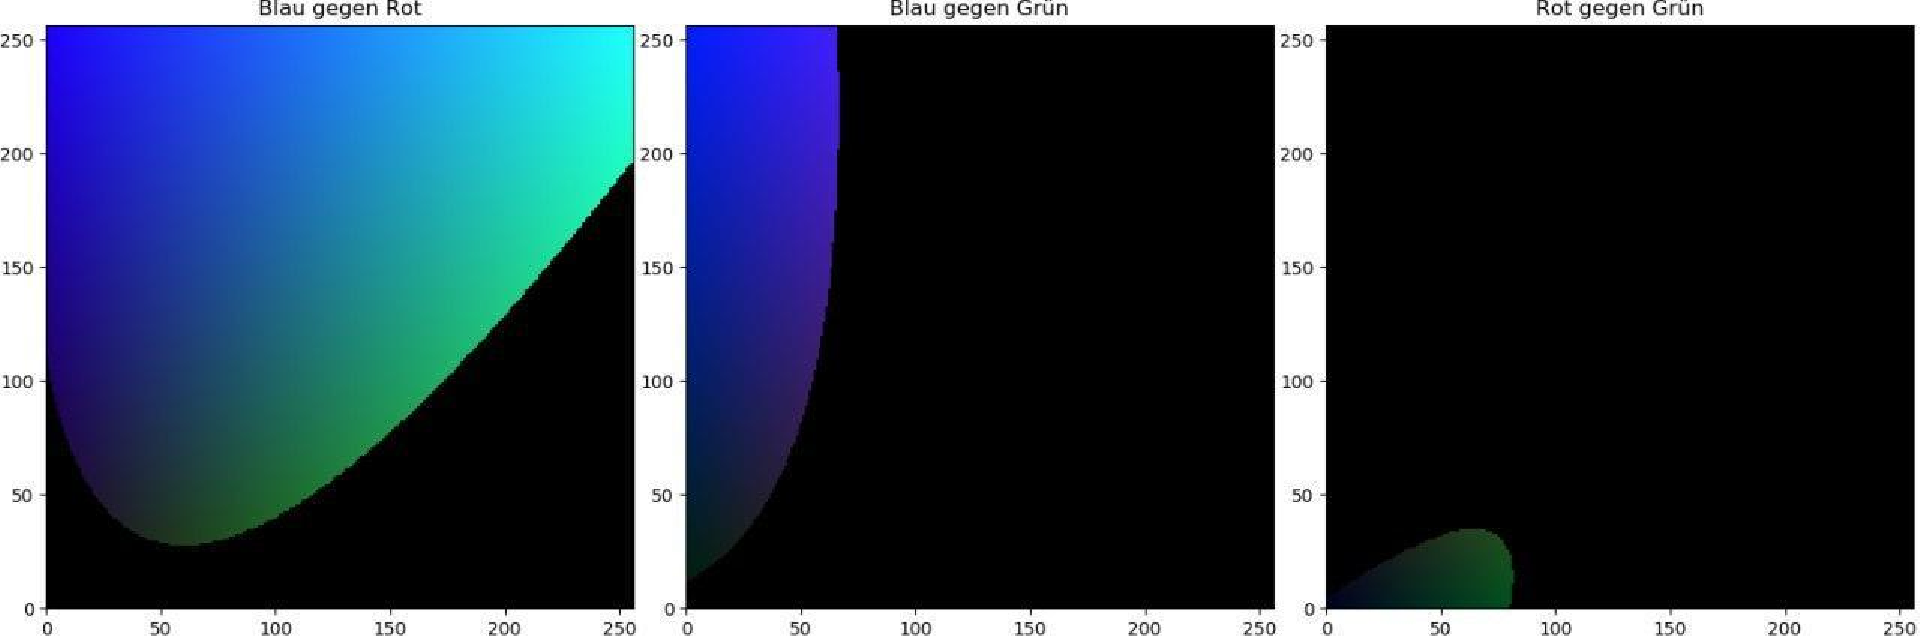
\includegraphics[width=\textwidth]{content/colorcuts1.pdf}

      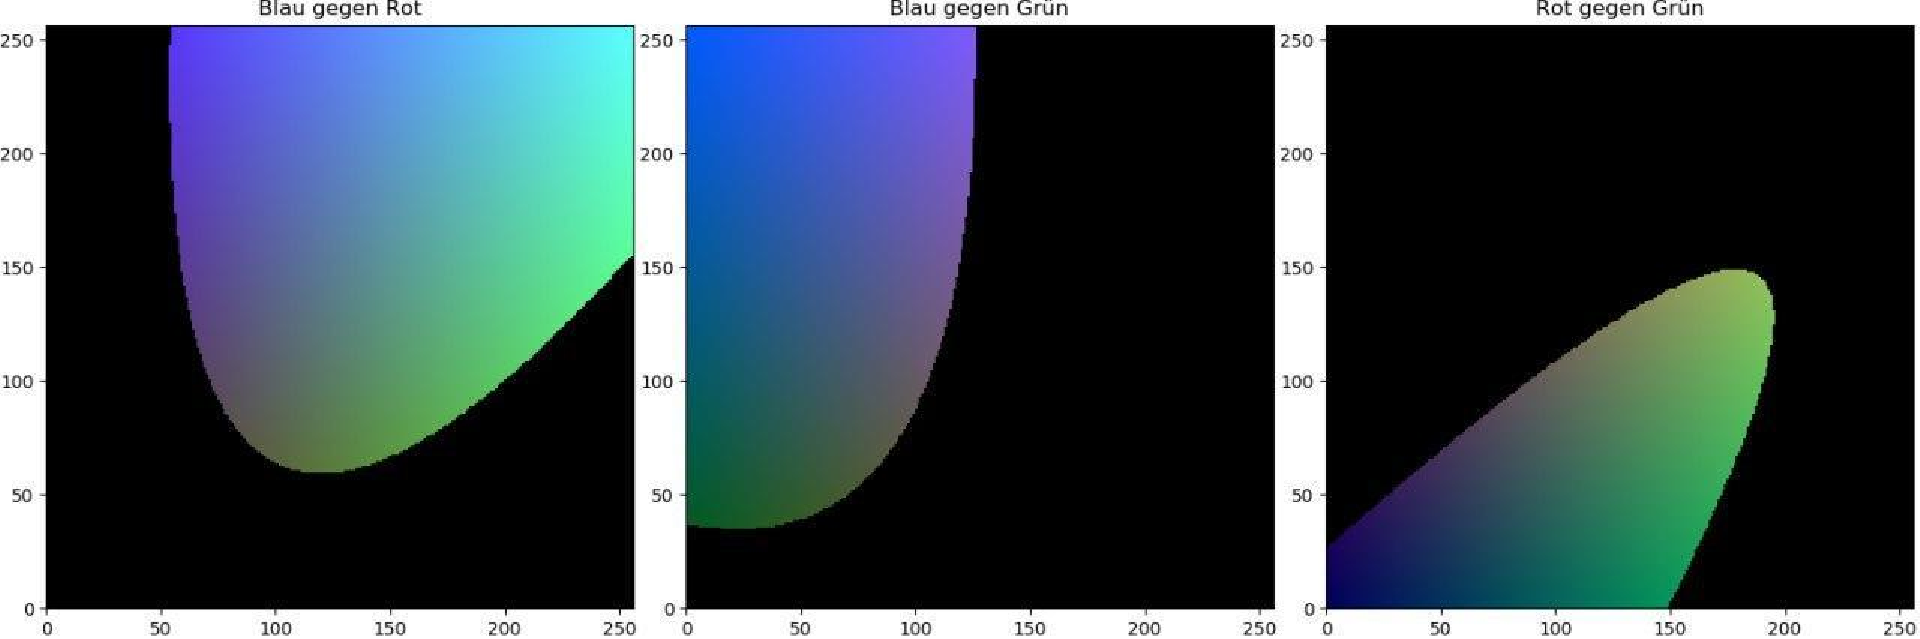
\includegraphics[width=\textwidth]{content/colorcuts2.pdf}

      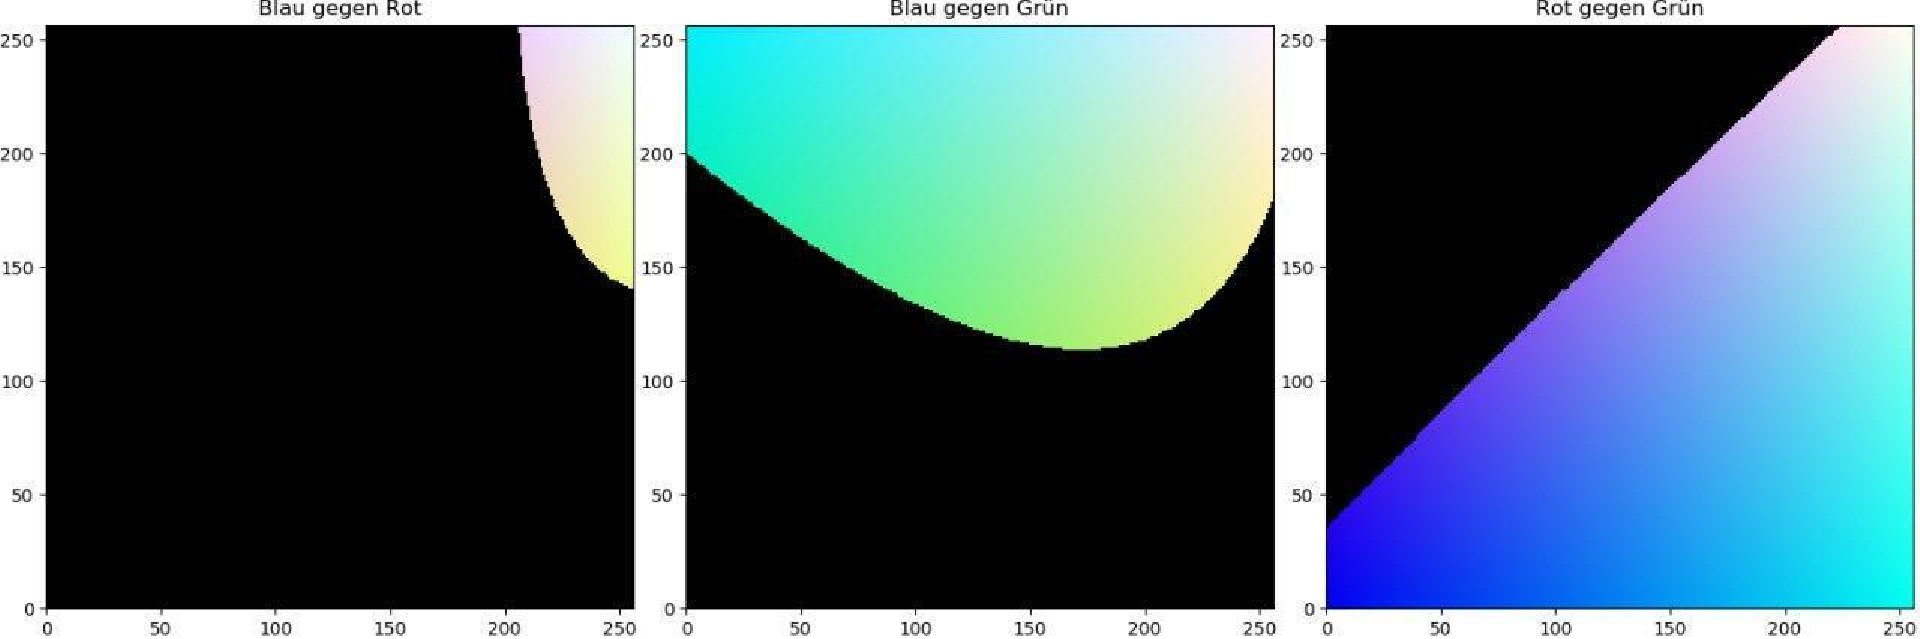
\includegraphics[width=\textwidth]{content/colorcuts3.pdf}
    \end{column}
    \begin{column}{0.5\textwidth}
      Histogrammieren der Cuts

      \centering
      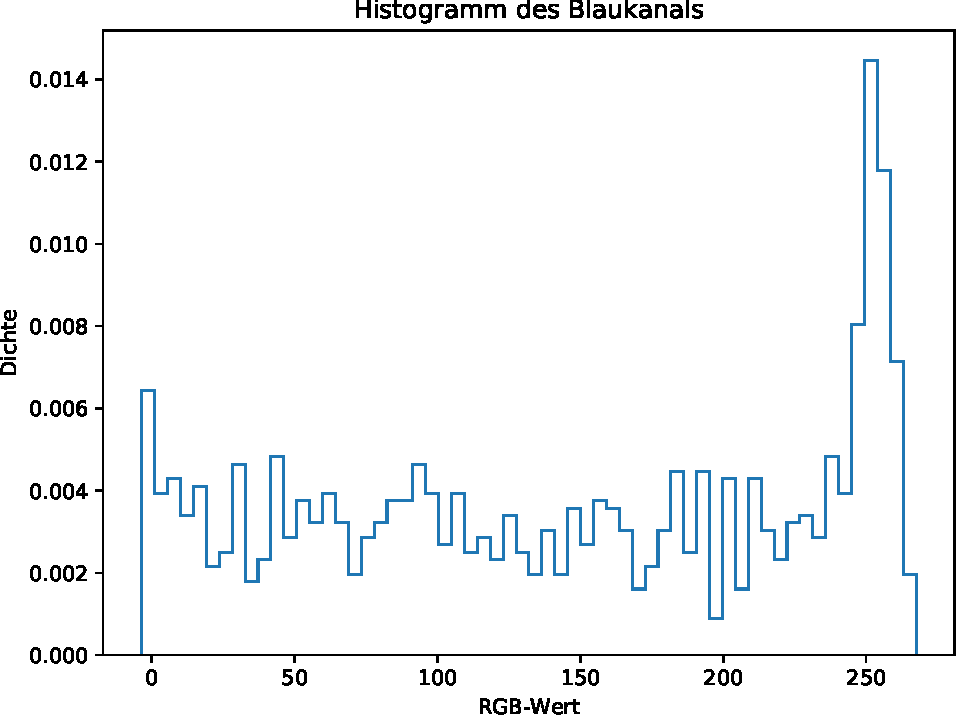
\includegraphics[width=\textwidth]{content/hist.pdf}
    \end{column}
  \end{columns}
  \centering

  $\Rightarrow$ \SI{40}{\percent} Genauigkeit
\end{frame}
